\section{乱数とは}
乱数とはランダムな数のことを言い,乱数の数列を乱数列と言います.
乱数列は生成した数から次に生成する数を予測することができないことや,
非周期的などの性質があります.
乱数は原子の崩壊による放射線の輻射レベルや時間間隔,
抵抗器の熱雑音などの物理現象の中で観測することが出来ます.
自然現象から観測できる乱数を真の乱数または自然乱数などと言います.

乱数は現在,数値計算や物理現象のシミュレーション,
暗号化などに使われており,計算機上で生成する需要が高まっています.
しかし,計算機は決定的オートマトンなため,数値の計算は
確率的にしか行えず,真の乱数を生成することができません.
よって,現在は統計的に真の乱数と近似の性質を持つ数列を
生成する方法があり,その方法を疑似乱数アルゴリズムと言い,
疑似乱数アルゴリズムによって生成された数を疑似乱数と言います.

現在,世に出回っている疑似乱数アルゴリズムは様々あります.
これは今まで研究されてきたアルゴリズムに何かしらの問題があるからです.
偏りが出たり,パターンがあったり様々です.
また,疑似乱数には周期があります.
一定の数の乱数を出力したらまた,
最初から同じ疑似乱数列を出力し始めます.
現在は計算機のスペックも高くなりより複雑なシミュレーションを
行えるようになりました.
その為,用いられる疑似乱数の数が従来のアルゴリズムでは
周期を上回る危険性もありました.
周期を伸ばすことも新しい疑似乱数アルゴリズムを開発する理由の一つです.

乱数の歴史は長く,現在では様々なプログラミング言語に
標準で実装されています.
しかし,標準で実装されている疑似乱数アルゴリズムも
言語によってまちまちです.昔からあるプログラミング言語の場合,
標準実装されているアルゴリズムも昔のものである場合が多く,
いわゆる問題点があるアルゴリズムであることもあります.
本章ではプログラミング言語の中でも\LaTeX に実装されている
疑似乱数アルゴリズムについて解説し,周期性や偏りについて検証していきます.
\section{乱数生成コマンド}
\LaTeX のパッケージに固定小数演算ができるFPパッケージがあります.
\subsection{固定小数演算}
\TeX ,\LaTeX は共に整数の演算は可能ですが,小数点を含む計算は行うことができません(寸法を除く).
固定小数点の演算をすることを目的としてあるのがFPパッケージです.
\subsection{乱数を出力するFPrandomコマンド}
fpパッケージの中には上記以外にも$0\sim 1$の範囲の疑似乱数を出力するFPrandomというコマンドがあります.
FPseedでシード値を決めてからFPrandomを使って変数に乱数を格納します.
\begin{texcode}
\FPseed = 156
\FPrandom{\result}
\FPprint{\result}
\end{texcode}

\section{FPrandomの乱数生成アルゴリズムを調べる}
\subsection{目的}
今回はFPrandomに使われている疑似乱数がいわゆる多くの問題点がある昔のアルゴリズムかどうかを調べる為に行います.

\subsection{ソースを読む}
それではfpパッケージのソースを読んでいきます.
しかし,実際にはfpパッケージ本体が内部的に呼び出しているfp-randomパッケージのソースを読んでいきます.

\subsubsection{コメントに正解が書いてあった}
22行目からFPrandomの定義が始まります.その直後,コメントが長く続いています.
コメントには次のようなことが書かれていました.
\begin{quote}
Algorithm reproduce from a very old Fortran program (unknown origin!)
\end{quote}
どうやら大昔のFortranの疑似乱数アルゴリズムを\TeX に起こしたものがFPrandomの正体みたいですね.
更にその下のコメントにはFortranで書かれた疑似乱数アルゴリズムらしきものがあります.
これを読んでいけばどんなアルゴリズムが使われているか分かりますがそれではつまらないので
コメントを抜けた後の\TeX で書かれた疑似乱数アルゴリズムの方を見ていきましょう.

\subsubsection{\TeX のマクロで実装された疑似乱数アルゴリズム}
\begin{texcode}
\ifnum\FPseed=0%
     \FPseed=123456789%
     \FP@debug{random: seed value undefined! We will used \the\FPseed.%
        Define it if you want to generate a different sequence of random numbers.}%
\else%
     \FP@debug{random: seed value used: \the\FPseed}%
\fi%
\end{texcode}
これはシードを指定してるかどうかを判定してしてない場合123456789をシードとするというマクロですね.
次見ていきます.
\begin{texcode}
\FP@xia=\FPseed%
\divide\FP@xia by 127773%
\FP@xib=\FP@xia%
\multiply\FP@xib by 127773%
\advance\FP@xib by -\FPseed%
\FP@xib=-\FP@xib%
\multiply\FP@xia by 2836%
\FPseed=\FP@xib%
\multiply\FPseed by 16807%
\advance\FPseed by -\FP@xia%
\end{texcode}
このアルゴリズムのコアとなる乱数の計算ですね.\TeX で書いてる為ごちゃごちゃしていますが
数式で表すと以下のようになります.

\begin{equation}\label{eq:LaTeXLGC}
S_{n+1} = - \frac{S_n}{127773}\times 2836 + 16807(S_n \bmod 127773)
\end{equation}
$S_n$が$n$番目に出力した乱数で$S_{n+1}$は$n+1$番目に出力する乱数です.つまり漸化式になっています.
線形合同法の漸化式と似ています.線形合同法はC言語のrand関数に
採用されているアルゴリズムですが
多くの問題点が発見されていて現在は非推奨となっています.
線形合同法の式は以下の通りです.
\begin{equation}\label{eq:LGC}
S_{n+1}=(A\times S_n + B) \bmod M \quad \textrm{(A,B,Mは定数)}
\end{equation}
式\eqref{eq:LaTeXLGC}の$16807(S_n \bmod 127773)$の部分が
式\eqref{eq:LGC}の定数$B$に対応しており,
更に乱数を含む形になっています.
式\eqref{eq:LaTeXLGC}の$M$にあたる変数が式\eqref{eq:LGC}に
ありませんが,これはオーバーフローを利用することによって省略しています.

次のコードを見ていきます.
\begin{texcode}
 \ifnum\FPseed>0%
  \else%
      \advance\FPseed by 2147483647%
  \fi%
  \FPdiv\FP@tmpa{\the\FPseed}{2147483647}%
  \global\let\FP@tmp\FP@tmpa%
  \global\FPseed=\FPseed%
\end{texcode}
乱数の正規化を行っています.$2147483647(=2^{31}-1)$がこの乱数列における最大値$M$で
この時点で$n+1$番目の乱数が負の値の場合は$M$を乱数に足します.
その後FPdivと呼ばれる小数の割り算ができるマクロによって乱数を$M$で割り,乱数を$0\sim 1$の範囲の値に正規化しています.
\begin{texcode}
  \let#1\FP@tmp%
\end{texcode}
最後に,FPrandomの第一引数に算出した乱数を代入して終了です.
\subsubsection{実際に出力してみる}
前節でFPrandomは線形合同法を改変したものが用いられていることが分かりました.
しかし,線形合同法は実装が簡単にできる分,構造が単純で,
偏りが出たり,周期が短いことが問題となっています.
この節では,その問題点がFPrandomコマンドにも起こるかどうかを検証していきます.
まずは分かりやすい規則性についてですが,線形合同法の代表的な
規則性として「偶数と奇数が交互に生成される」という性質を持っています.
以下の\LaTeX のソースをタイプセットすると,
結果が分かります.
\begin{texcode}
  \documentclass[dvipdfmx,uplatex]{jsarticle}
  \usepackage[nomessages]{fp}
  \usepackage{ifthen}
  \FPseed = 1
  \begin{document}
  生成した回数 \quad 生成した乱数 \\
  0 \quad \the\FPseed \\
  \newcounter{mycounter}
  \setcounter{mycounter}{0}

  \whiledo{\value{mycounter}<1000}{%
  \FPrandom{\result}%
  \addtocounter{mycounter}{1}
  \arabic{mycounter}\quad\the\FPseed\\%
  }
  \end{document}
\end{texcode}
タイプセットしてみると,偶数と奇数は交互に出てきません.
よって,規則性については線形合同法から改良されています.

次に周期性ですが,線形合同法の最大周期は$M-1$です.
FPrandomは$M=2147483647$なので周期は$2147483646$となります.
つまり,FPrandomコマンドを$M$回呼び出すと最初の乱数と一致することになります.
\LaTeX で検証したいところですが,FPrandomコマンドはとても遅く,
また,\TeX のメモリ制限によって,最後まで出力できないので.
Pythonで検証をしてみます.
\captionof{listing}{Pythonで実装したFPrandomのアルゴリズム}
\inputpython{\keisukeasset/latex_lcg.py}
\captionof{listing}{周期性の検証プログラム}
\inputpython{\keisukeasset/periodicity.py}
時間がかかりますが,$M$回乱数を生成しても,
最初の乱数と一致しないので,周期も通常の線形合同法に
比べて長くなっているようです.
具体的な周期の長さについては検証する時間がありませんでしたが,
またいつか,検証したいと思います.

次に偏りについての検証です.線形合同法は3次元以上の
乱数の一様性については保証されていません.
通常の線形合同法で生成した乱数を3次元空間上に
プロットすると,空間上にプロット点で構成された層の
ような模様が浮かび上がり,点が一様にプロットされません.
FPrandomではこのような問題点がないかを検証します.
周期性と同じくPythonで検証していきます.
\captionof{listing}{偏りの検証プログラム}
\label{lst:bias}
\inputpython{\keisukeasset/bias.py}
Listing \ref{lst:bias}で書き込まれたcoodinates.datを
gnuplotでプロットしてみると,
図\ref{fig:bias}のようになります.
\begin{figure}[htbp]
  \centering
  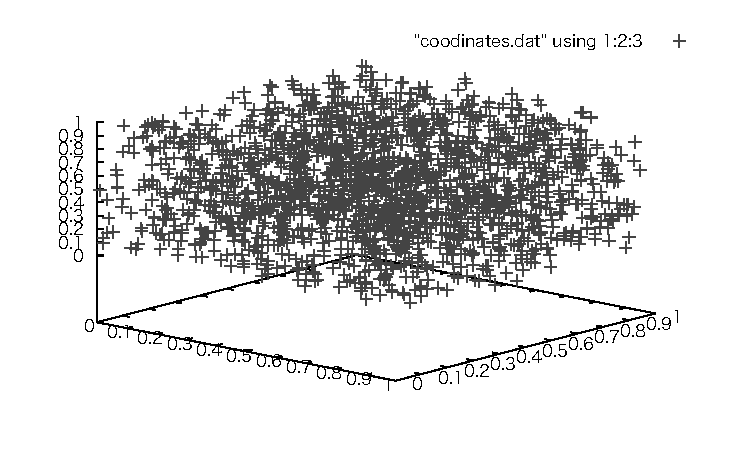
\includegraphics[width=60mm]{\keisukeasset/keisuke495500_graph_gray.pdf}
  \caption{FPrandomのアルゴリズムを元に2000個の乱数を3次元上にプロットしたグラフ}
  \label{fig:bias}
\end{figure}
通常の線形合同法と違い,かなり一様に分布しているように見えます.
偏りについても特に問題がないように思えます.

\section{おわりに}
今回,FPrandomの疑似乱数生成アルゴリズムについての検証を行いました.
しかし,今回の検証では特に問題がありませんでした.
次回は,具体的な周期の長さや\LaTeX の他の乱数を生成する
パッケージ(lcgパッケージ)などについての検証も行っていきたいと思います.
